% Options for packages loaded elsewhere
\PassOptionsToPackage{unicode}{hyperref}
\PassOptionsToPackage{hyphens}{url}
\documentclass[
]{ltjsarticle}
\usepackage{xcolor}
\usepackage{amsmath,amssymb}
\setcounter{secnumdepth}{-\maxdimen} % remove section numbering
\usepackage{iftex}
\ifPDFTeX
  \usepackage[T1]{fontenc}
  \usepackage[utf8]{inputenc}
  \usepackage{textcomp} % provide euro and other symbols
\else % if luatex or xetex
  \usepackage{unicode-math} % this also loads fontspec
  \defaultfontfeatures{Scale=MatchLowercase}
  \defaultfontfeatures[\rmfamily]{Ligatures=TeX,Scale=1}
\fi
\usepackage{lmodern}
\ifPDFTeX\else
  % xetex/luatex font selection
\fi
% Use upquote if available, for straight quotes in verbatim environments
\IfFileExists{upquote.sty}{\usepackage{upquote}}{}
\IfFileExists{microtype.sty}{% use microtype if available
  \usepackage[]{microtype}
  \UseMicrotypeSet[protrusion]{basicmath} % disable protrusion for tt fonts
}{}
\makeatletter
\@ifundefined{KOMAClassName}{% if non-KOMA class
  \IfFileExists{parskip.sty}{%
    \usepackage{parskip}
  }{% else
    \setlength{\parindent}{0pt}
    \setlength{\parskip}{6pt plus 2pt minus 1pt}}
}{% if KOMA class
  \KOMAoptions{parskip=half}}
\makeatother
\usepackage{longtable,booktabs,array}
\newcounter{none} % for unnumbered tables
\usepackage{calc} % for calculating minipage widths
% Correct order of tables after \paragraph or \subparagraph
\usepackage{etoolbox}
\makeatletter
\patchcmd\longtable{\par}{\if@noskipsec\mbox{}\fi\par}{}{}
\makeatother
% Allow footnotes in longtable head/foot
\IfFileExists{footnotehyper.sty}{\usepackage{footnotehyper}}{\usepackage{footnote}}
\makesavenoteenv{longtable}
\usepackage{graphicx}
\makeatletter
\newsavebox\pandoc@box
\newcommand*\pandocbounded[1]{% scales image to fit in text height/width
  \sbox\pandoc@box{#1}%
  \Gscale@div\@tempa{\textheight}{\dimexpr\ht\pandoc@box+\dp\pandoc@box\relax}%
  \Gscale@div\@tempb{\linewidth}{\wd\pandoc@box}%
  \ifdim\@tempb\p@<\@tempa\p@\let\@tempa\@tempb\fi% select the smaller of both
  \ifdim\@tempa\p@<\p@\scalebox{\@tempa}{\usebox\pandoc@box}%
  \else\usebox{\pandoc@box}%
  \fi%
}
% Set default figure placement to htbp
\def\fps@figure{htbp}
\makeatother
\setlength{\emergencystretch}{3em} % prevent overfull lines
\providecommand{\tightlist}{%
  \setlength{\itemsep}{0pt}\setlength{\parskip}{0pt}}
\usepackage{bookmark}
\IfFileExists{xurl.sty}{\usepackage{xurl}}{} % add URL line breaks if available
\urlstyle{same}
\hypersetup{
  hidelinks,
  pdfcreator={LaTeX via pandoc}}

\author{}
\date{}

\begin{document}

\section{論文7：配置統計と関係的読み出し}\label{ux8ad6ux65877ux914dux7f6eux7d71ux8a08ux3068ux95a2ux4fc2ux7684ux8aadux307fux51faux3057}

\subsection{排他統計の導出・安定種スペクトル・無時間分岐比・関係的幾何の誕生とそのホログラフィック読み出し}\label{ux6392ux4ed6ux7d71ux8a08ux306eux5c0eux51faux5b89ux5b9aux7a2eux30b9ux30daux30afux30c8ux30ebux7121ux6642ux9593ux5206ux5c90ux6bd4ux95a2ux4fc2ux7684ux5e7eux4f55ux306eux8a95ux751fux3068ux305dux306eux30dbux30edux30b0ux30e9ux30d5ux30a3ux30c3ux30afux8aadux307fux51faux3057}

著者: 木原 範昭 (Noriaki Kihara)\\
所属: WF System Co., Ltd.\\
ORCID: 0009-0004-6753-4020\\
版: v0.2\\
日付: 2026 年 6 月\\
DOI（本版）: 10.5281/zenodo.20640459\\
Concept DOI: 10.5281/zenodo.20640458\\
ライセンス: CC BY 4.0

\begin{center}\rule{0.5\linewidth}{0.5pt}\end{center}

\subsection{要旨}\label{ux8981ux65e8}

本稿は、逆数双対モデル（論文1--6）に\textbf{配置読み}を導入する：分裂後の断片は共有された親格子の占有セルであり、状態とは占有セルの集合である。この最小の埋め込み仮説から、次が導出される。

第一に、\textbf{排他統計}：状態が集合である以上、断片に「どれがどれか」のラベルは存在せず、同一セルの二重占有は非重複＝直交定理（論文5）により不可能である。区別不能性と排他原理は、仮定ではなく定理的帰結となる。

第二に、\textbf{安定種スペクトル}：排他から殻容量則 \(n_m\le c(m)\)
が従い、奇数分割と容量則による許容崩壊チャネルの全数スキャン（\(s\le25\)）の結果、\(s=1,3,5\)
は\textbf{絶対安定}（チャネルが存在しない）、崩壊の敷居は \(s=7\)
であることが確定する。モデルは初めて安定状態のスペクトルを持つ。

第三に、\textbf{無時間分岐比}：「いつ・何が引き金で崩壊するか」という問いは、時間＝イベント列であるこのモデルでは悪設定であり、引き金の不在（自発性）は時間の構成原理である。予言可能なのはチャネル間の相対重み（分岐比）であり、\(s=9\)
では許容2チャネルの配置数え上げから一意の比
\((5,3,1):(3,3,3)=192:56\)（77.4\% : 22.6\%）が得られる。

第四に、\textbf{関係的幾何の誕生と読み出し}：単独の断片の配置は \(B_4\)
ゲージで非観測量だが、2個以上で初めて占有セル間の内積＝角度がゲージ不変量になる。この関係データが
\(\lambda\)
側の記録（干渉パターンの強度）のみから完全に読み出せることを示す：\(s=9\)
崩壊終配置の5つの関係クラスは、多重度込みパワースペクトルだけで完全分離し（全248配置についての定理）、識別に要する全データは\textbf{単位記録1個分}で厳密に得られる（単位記録十分性定理）。振幅は
\(\sqrt2\)
の冪の離散アルファベットに乗り、読み出しはデジタル復号である。最小断片（零モード）を含むチャネルは配置の完全再構成を許す\textbf{ホログラフィック型}、含まないチャネルは関係のみの\textbf{干渉計的型}に分かれる。

最後に、排他則の帰結として、共有格子内では既存の占有が他の断片の崩壊チャネルを塞ぐ\textbf{閉塞効果}が生じること（崩壊チャネルの環境依存性）、および小さい系の無時間状態空間が有限閉集合として完全に列挙できることを示す。

\begin{center}\rule{0.5\linewidth}{0.5pt}\end{center}

\subsection{キーワード}\label{ux30adux30fcux30efux30fcux30c9}

排他原理、区別不能性、配置空間、安定スペクトル、分岐比、ゲージ不変量、関係的幾何、ホログラフィー、デジタル復号、選択則

\begin{center}\rule{0.5\linewidth}{0.5pt}\end{center}

\subsection{1. はじめに}\label{ux306fux3058ux3081ux306b}

論文6 {[}3{]} で確立した運動学（凍結定理・\(B_4\)
ゲージ・記録定理）は、複数の断片が共存する系を扱う準備である。本稿の問いは二つ：

\begin{enumerate}
\def\labelenumi{\arabic{enumi}.}
\tightlist
\item
  複数の断片はどんな統計に従うか ---
  区別可能か、同一セルを共有できるか。
\item
  断片たちの関係（距離・角度）は観測量か ---
  観測量なら、どの記録から読めるか。
\end{enumerate}

量子統計（Pauli の排他原理 {[}5{]}、Fermi--Dirac 統計
{[}6,7{]}）は標準理論では経験則ないし場の量子化の帰結として導入される。統計力学の等重率は公準である（基礎づけの議論として
Jaynes
{[}8{]}）。また、参照系なしには相対量のみが観測可能であるという視点は量子情報の文脈で体系化されている（Bartlett,
Rudolph \& Spekkens
{[}9{]}）。本稿はこれらの結果を\textbf{有限格子模型の中で全数検証可能な形で}再構成する：統計は配置読みから導出され、等重率はモデルの数え上げ原理として明示され、関係のみの観測可能性は記録定理（論文6）から従い、読み出しの具体的手続きはホログラフィー（Gabor
{[}10{]}）と構造的に同型の機構で与えられる。

\begin{center}\rule{0.5\linewidth}{0.5pt}\end{center}

\subsection{2.
配置読み（最小埋め込み仮説）}\label{ux914dux7f6eux8aadux307fux6700ux5c0fux57cbux3081ux8fbcux307fux4eeeux8aac}

\begin{quote}
\textbf{仮説（配置読み）}:
分裂後の断片は、共有された親格子の占有セルである。断片の代表値はその占有セルの
\(r_{\max}(k)^2\)、すなわちエネルギー様量＝周波数空間内の動径位置。状態＝占有セルの\textbf{集合}。
\end{quote}

使用部品はすべて既存である：格子（論文2 {[}4{]}）、代表化（論文5 {[}2{]}
§6.4）、非重複＝直交（論文5 §5）、二値占有。論文4 {[}1{]} の有限 \(R'\)
分裂表現を、共有された親格子の占有として具体化した形である。新規部品はゼロの最小構成だが、埋め込みの\textbf{選択}であることを明示する（独立な検証は
§6 の読み出し定理が与える）。

\subsubsection{2.1
排他統計の導出}\label{ux6392ux4ed6ux7d71ux8a08ux306eux5c0eux51fa}

状態が占有セルの集合である以上、(i)
断片に個体ラベルは存在しない（集合に重複なし）、(ii)
同一セルの二重占有は直交定理により不可能。

\begin{quote}
\textbf{帰結}:
断片は区別不能な占有であり、排他原理に従う。統計は仮定ではなく、二値占有＋直交性の定理的帰結である。
\end{quote}

\begin{center}\rule{0.5\linewidth}{0.5pt}\end{center}

\subsection{3.
殻容量則と安定種スペクトル}\label{ux6bbbux5bb9ux91cfux5247ux3068ux5b89ux5b9aux7a2eux30b9ux30daux30afux30c8ux30eb}

\subsubsection{3.1 容量則}\label{ux5bb9ux91cfux5247}

各殻 \(m\) のセル数は \(c(m)=1,8,24,40,64,96,96,144,\ldots\)（論文5
§8）。排他より

\[
n_m\le c(m)
\]

（ラベル \(m\) の断片数は殻容量以下）。特に
\(c(1)=1\)：\textbf{ラベル1の断片は系に1個まで}。

\subsubsection{3.2
安定種スペクトル}\label{ux5b89ux5b9aux7a2eux30b9ux30daux30afux30c8ux30eb}

奇数分割（論文5の整合条件）＋容量則による許容チャネルの全数スキャン：

{\def\LTcaptype{none} % do not increment counter
\begin{longtable}[]{@{}rll@{}}
\toprule\noalign{}
\(s\) & 許容チャネル数 & 備考 \\
\midrule\noalign{}
\endhead
\bottomrule\noalign{}
\endlastfoot
1, 3, 5 & \textbf{0（絶対安定）} & \\
7 & 1（(3,3,1) のみ） & 崩壊の敷居 \\
9 & 2（(5,3,1), (3,3,3)） & \\
11 & 3 & \\
13 & 5 & 最小5体チャネルを含む \\
25 & 37 & チャネル数は \(s\) と共に急増 \\
\end{longtable}
}

\begin{quote}
\textbf{主結果}: \(s=1,3,5\)
は運動学的にチャネルが存在せず絶対安定。崩壊の敷居は
\(s=7\)。容量則は素朴な7チャネル（\(s=9\)）のうち5本（複数の \(s=1\)
を含むもの等）を排除する。
\end{quote}

\begin{figure}
\centering
\pandocbounded{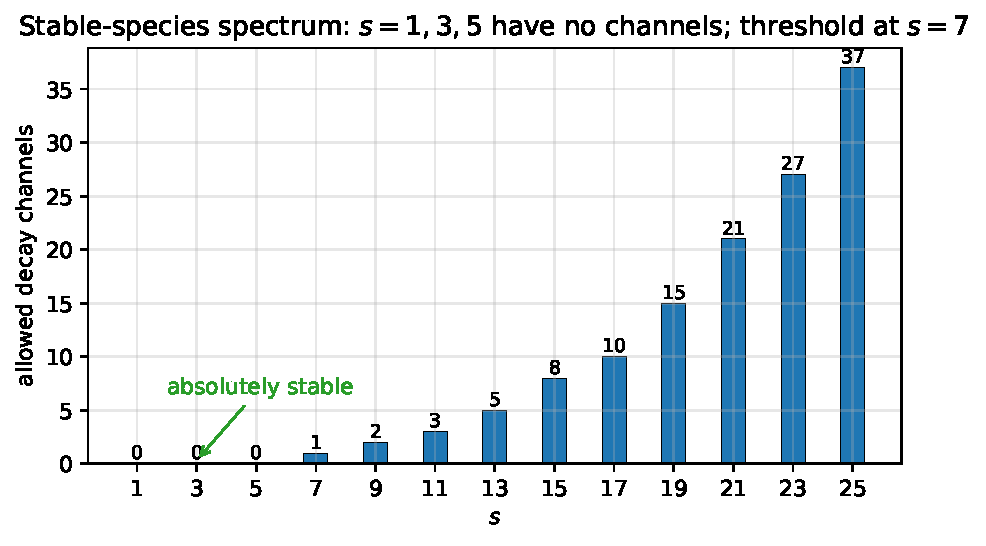
\includegraphics[keepaspectratio,alt={Figure 1. Stable-species spectrum and the decay threshold}]{figure_paper7_1_stable_species.pdf}}
\caption{Figure 1. Stable-species spectrum and the decay threshold}
\end{figure}

\textbf{図1.
安定種スペクトル：許容崩壊チャネル数（奇数分割＋容量則、全数）。\(s=1,3,5\)
はチャネルゼロ（絶対安定）、敷居は \(s=7\)。}

\subsubsection{3.3 終端の系}\label{ux7d42ux7aefux306eux7cfb}

カスケードの最終段 \(3\to(1,1,1)\) は \(c(1)=1\)
により禁止される。よって\textbf{全1状態は到達不能}であり、分割カスケードの終端個体群は安定種
\(\{1,3,5\}\)
の混合である。また一つの格子内での最大分散は「最下殻から1セルずつ詰める」配置（フェルミ海型、\(n_{\max}\sim S^{2/3}\)）となる。

\begin{center}\rule{0.5\linewidth}{0.5pt}\end{center}

\subsection{4. 無時間分岐比}\label{ux7121ux6642ux9593ux5206ux5c90ux6bd4}

\subsubsection{4.1
問いの再設定}\label{ux554fux3044ux306eux518dux8a2dux5b9a}

「なぜ安定が自発的に崩れるのか」を「いつ・何が引き金で」と読むなら、崩壊の前に流れる背景時間が要る。本モデルでは時間＝イベント列（論文6）であり、イベントの前に時間はない。\textbf{引き金の不在＝自発性は、時間がイベントから構成されることの表現である。}
良設定の問いは (i) どのチャネルが開いているか（§3 で完了）、(ii)
チャネル間の相対重みは何か、の二つに分解され、(ii)
は静的数え上げで予言可能である。

\subsubsection{\texorpdfstring{4.2 \(s=9\)
の一意分岐比}{4.2 s=9 の一意分岐比}}\label{s9-ux306eux4e00ux610fux5206ux5c90ux6bd4}

生き残る2チャネルの配置数（\(c(1)=1\), \(c(3)=8\), \(c(5)=24\)）：

\[
W(5,3,1)=24\times8\times1=192\;(77.4\%),\qquad
W(3,3,3)=\binom{8}{3}=56\;(22.6\%)
\]

\begin{quote}
配置の等重率（数え上げ原理）の下で、分岐比は一意である。等重率自体の地位については
§8 で論じる。
\end{quote}

\begin{figure}
\centering
\pandocbounded{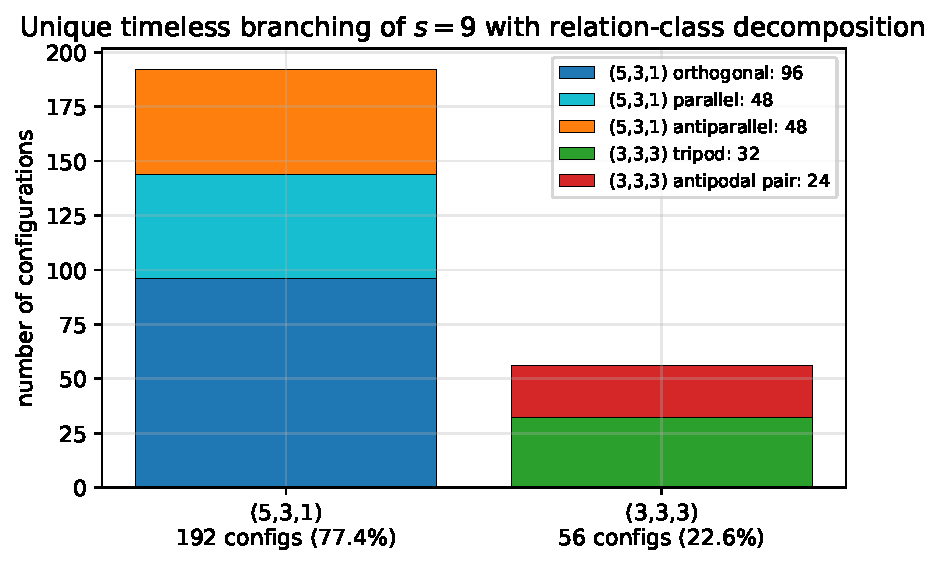
\includegraphics[keepaspectratio,alt={Figure 2. Unique timeless branching of s=9 with relation-class decomposition}]{figure_paper7_2_branching.pdf}}
\caption{Figure 2. Unique timeless branching of s=9 with relation-class
decomposition}
\end{figure}

\textbf{図2. \(s=9\)
の一意無時間分岐比（192:56＝77.4\%:22.6\%）と5関係クラスへの分解（248配置の内訳）。}

\subsubsection{4.3
閉塞効果（崩壊チャネルの環境依存性）}\label{ux9589ux585eux52b9ux679cux5d29ux58caux30c1ux30e3ux30cdux30ebux306eux74b0ux5883ux4f9dux5b58ux6027}

共有格子では、既存の占有が他の断片のチャネルを塞ぐ。例：断片組
\(\{7,3,1\}\) では、\(7\) の唯一のチャネル \((3,3,1)\)
は原点（\(c(1)=1\)）が占有済みのため\textbf{閉塞}され、\(7\)
は環境により安定化される。\(\{9,3,1\}\) では \(9\) の \((5,3,1)\)
が閉塞され、分岐比が環境で 100\% \((3,3,3)\)
に改変される。\textbf{安定性・分岐比は孤立系の属性ではなく配置の属性である。}

\subsubsection{4.4
有限閉集合としての状態空間}\label{ux6709ux9650ux9589ux96c6ux5408ux3068ux3057ux3066ux306eux72b6ux614bux7a7aux9593}

小さい \(S\) の到達可能配置は完全に列挙できる（例：\(S_0=9\) は
\(\{9\},\{5,3,1\},\{3,3,3\}\) の3配置、ゲージ不変状態数
\(1+3+2=6\)）。無時間の状態空間が有限の遷移系として手に取れることは、本モデルの検証可能性の核である。

\begin{center}\rule{0.5\linewidth}{0.5pt}\end{center}

\subsection{5.
関係的幾何の誕生}\label{ux95a2ux4fc2ux7684ux5e7eux4f55ux306eux8a95ux751f}

断片1個の配置（殻上の位置）は \(B_4\)
ゲージで純粋に非観測量である（論文6 §4）。\(B_4\subset O(4)\)
は内積を保存するから、\textbf{2個以上で初めて、占有セル間の内積＝角度がゲージ不変量として観測可能になる。}

\(s=9\) の崩壊終配置248通り（\((5,3,1)\): 192、\((3,3,3)\):
56）は、\(B_4\) 軌道分解により5つの関係クラスに分かれる：

{\def\LTcaptype{none} % do not increment counter
\begin{longtable}[]{@{}llrr@{}}
\toprule\noalign{}
クラス & 不変量 & 配置数 & 比率 \\
\midrule\noalign{}
\endhead
\bottomrule\noalign{}
\endlastfoot
\((5,3,1)\) 直交型 & \(\langle v_5,v_3\rangle=0\) & 96 & 38.7\% \\
\((5,3,1)\) 平行型 & \(+1\) & 48 & 19.4\% \\
\((5,3,1)\) 反平行型 & \(-1\) & 48 & 19.4\% \\
\((3,3,3)\) 三脚型 & 3軸直交 & 32 & 12.9\% \\
\((3,3,3)\) 対蹠対型 & 対蹠対を含む & 24 & 9.7\% \\
\end{longtable}
}

単独の断片に位置はなく、\textbf{配置の相対構造が最初の内在的幾何観測量}である。

\begin{center}\rule{0.5\linewidth}{0.5pt}\end{center}

\subsection{\texorpdfstring{6. \(\lambda\)
側読み出し：関係クラスのホログラフィック識別}{6. \textbackslash lambda 側読み出し：関係クラスのホログラフィック識別}}\label{lambda-ux5074ux8aadux307fux51faux3057ux95a2ux4fc2ux30afux30e9ux30b9ux306eux30dbux30edux30b0ux30e9ux30d5ux30a3ux30c3ux30afux8b58ux5225}

\subsubsection{6.1
読み出しモデルと記録の構造}\label{ux8aadux307fux51faux3057ux30e2ux30c7ux30ebux3068ux8a18ux9332ux306eux69cbux9020}

記録定理（論文6）により、観測量はすべて \(\lambda\)
側の記録として読めなければならない。各占有セルに辞書の実定在波
\(\Phi_k\)（論文5）を対応させ、配置の \(\lambda\) 側記録を強度
\(I(x)=\Psi(x)^2\)、\(\Psi=\sum_{k}\Phi_k\)
とする。積和公式により、\textbf{\(\lambda\)
側記録＝配置の自己相関スペクトル}であり、交差項は占有セルの対ごとの和・差ベクトルに乗る。

\subsubsection{6.2
5クラス完全分離（全248配置の定理）}\label{ux30afux30e9ux30b9ux5b8cux5168ux5206ux96e2ux5168248ux914dux7f6eux306eux5b9aux7406}

多重度・振幅込みのパワースペクトルの（ノルム²:
本数）データだけで、5クラスは完全に分離する：直交
\((1{:}1,\,3{:}4)\)、平行 \((1{:}2,\,5{:}2)\)、反平行
\((1{:}1,\,5{:}2)\)、三脚 \((2{:}6)\)、対蹠対
\((2{:}4)\)。ピーク強度（\(19.49/19.49/11.90/18/11.66\)）は独立な整合チェックである。枝・軸・符号の選択に依らない閉形式により、\textbf{全248配置でクラス内一定}が定理として成立する。

\begin{figure}
\centering
\pandocbounded{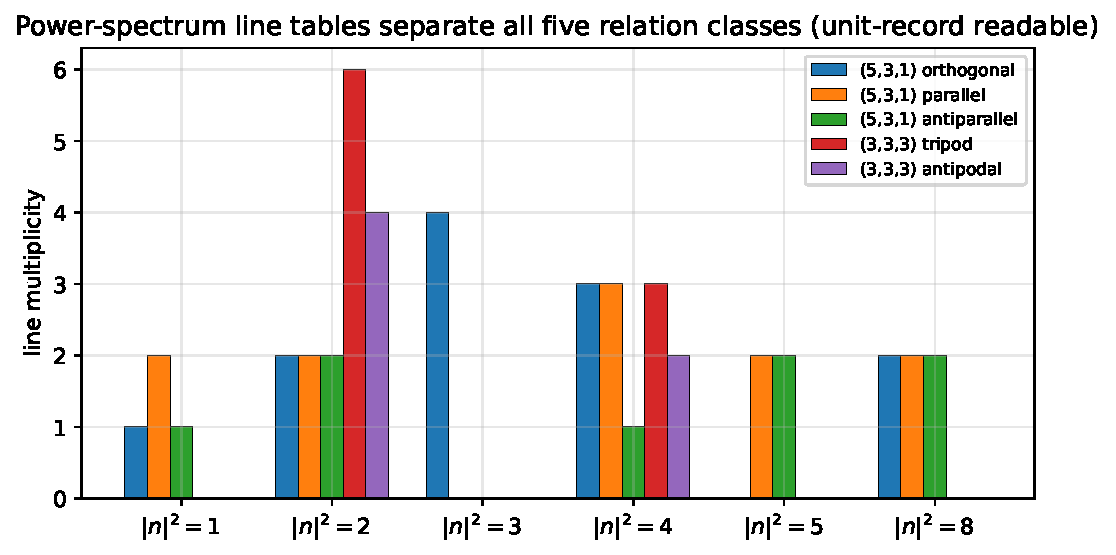
\includegraphics[keepaspectratio,alt={Figure 3. Complete line tables of the five relation classes}]{figure_paper7_3_line_tables.pdf}}
\caption{Figure 3. Complete line tables of the five relation classes}
\end{figure}

\textbf{図3.
5関係クラスの完全線テーブル：多重度込みパワースペクトル（ノルム²:
本数）のみで完全分離する --- 単位記録1個分で読める全データ。}

\subsubsection{6.3
単位記録十分性定理}\label{ux5358ux4f4dux8a18ux9332ux5341ux5206ux6027ux5b9aux7406}

干渉強度のスペクトル線は交差項・自己項とも整数周波数ベクトルに乗り、整数周波数モードは単位セル上で厳密に直交する。したがって：

\begin{quote}
\textbf{単位セル1個分の \(\lambda\)
記録から、全スペクトル線の振幅が厳密に決定できる。}
必要なのは超分解能ではなく、単位記録の分解能ちょうどである。
\end{quote}

\(I(x)\) は軸あたり次数 ≤2 の三角多項式なので、軸あたり等間隔5点、計
\(5^4=625\)
点の格子サンプルで厳密に再構成できる（有限・構成的な読み出し手続き）。

\subsubsection{6.4
デジタル振幅アルファベット}\label{ux30c7ux30b8ux30bfux30ebux632fux5e45ux30a2ux30ebux30d5ux30a1ux30d9ux30c3ux30c8}

全線の振幅は離散集合 \(\{\tfrac12,1,\sqrt2,2,2\sqrt2\}=(\sqrt2)^j\)
に乗る。読み出しは約 ±20\%
の相対精度で足りる\textbf{デジタル復号}である。

\subsubsection{6.5
ホログラフィック型と干渉計的型}\label{ux30dbux30edux30b0ux30e9ux30d5ux30a3ux30c3ux30afux578bux3068ux5e72ux6e09ux8a08ux7684ux578b}

振幅 \(2\sqrt2\) の線は
\(2\Phi_0\Phi_k=2\Phi_k\)、すなわち成分波の線形転写であり、\(s=1\)
断片（零モード＝定数波）が存在する場合にのみ立つ。

\begin{itemize}
\tightlist
\item
  \textbf{\((5,3,1)\)
  型（参照あり）＝ホログラフィック}：線形転写から各断片のセル・枝まで配置を完全再構成できる。参照光を用いる
  Gabor のホログラフィー {[}10{]}
  と同一の構造である（構造対応であり同一視ではない）。
\item
  \textbf{\((3,3,3)\)
  型（参照なし）＝干渉計的}：対ごとの関係のみが読める。
\end{itemize}

最小断片の有無が記録の\textbf{情報クラス}を分ける。また強度の DC
成分は断片数 \(n\) に等しく、計数と \(Z_2\) パリティは \(\lambda\)
側で直読可能である。

\begin{center}\rule{0.5\linewidth}{0.5pt}\end{center}

\subsection{7.
本稿の主張範囲}\label{ux672cux7a3fux306eux4e3bux5f35ux7bc4ux56f2}

主張すること：(1) 配置読みからの排他統計の導出。(2) 殻容量則・安定種
\(\{1,3,5\}\)・敷居 \(s=7\)（全数スキャン）。(3) \(s=9\)
の一意分岐比（等重率の下で）。(4) 閉塞効果と有限閉状態空間。(5)
関係クラスの \(\lambda\)
側完全読み出し（全248配置定理・単位記録十分性・デジタルアルファベット・二つの情報クラス）。

主張しないこと：(1)
物理粒子・物質場との同一視（「排他」「統計」「分岐比」はモデル内の数え上げ構造の記述である）。(2)
遷移率・寿命の絶対値（動力学は射程外。予言は比に限る）。(3)
等重率の第一原理からの導出（§8）。(4)
配置読み以外の埋め込みの排除（読み出し定理は配置読みの独立テストへの合格であり、一意性の証明ではない）。

\begin{center}\rule{0.5\linewidth}{0.5pt}\end{center}

\subsection{8. 考察}\label{ux8003ux5bdf}

\textbf{等重率の地位。} 標準的な統計力学では等重率は公準である
{[}8{]}。本モデルでは、許容配置への等重率は「数え上げ以外の重み原理を導入しない」という最小性の表現であり、後続論文で、配置数え上げ以外の重みが運動学からは生成されないこと（重み導出の不可能性定理）を示す。

\textbf{関係のみの観測可能性。} 参照系の理論 {[}9{]}
が一般的枠組みで論じる「相対量のみが意味を持つ」という制約が、本モデルでは記録定理＋\(B_4\)
ゲージから具体的な読み出し手続き（§6）込みで実現する。特に、参照（零モード）の有無が読み出せる情報のクラスを切り替えるという機構は、ホログラフィーとヘテロダイン検波の構造を、数え上げモデルの内部で再現している。

\textbf{統計の出自。} Pauli の排他原理 {[}5{]}
は本モデルでは「集合であること＋直交性」に還元された。これは物理的フェルミオンの説明ではないが、「排他がどんな最小構造から生成されうるか」の一例を与える。

\begin{center}\rule{0.5\linewidth}{0.5pt}\end{center}

\subsection{9. 結論}\label{ux7d50ux8ad6}

配置読みという最小の埋め込み仮説から、排他統計・安定種スペクトル・一意の無時間分岐比・閉塞効果が導出され、関係的幾何（角度）が誕生し、その全情報が単位記録のデジタル復号で読み出せることが定理として確立した。とりわけ「識別に必要な分解能＝単位記録の分解能」という過不足ない一致は、配置読みが記録構造と整合する独立の証拠である。

論文8では、この統計の上に二つの会計（凝縮と膨張）を、論文9では複合体の安定性の波動的導出を構築する。

\begin{center}\rule{0.5\linewidth}{0.5pt}\end{center}

\subsection{付録：再現手順の要点}\label{ux4ed8ux9332ux518dux73feux624bux9806ux306eux8981ux70b9}

安定種スキャンは奇数分割の全列挙＋容量フィルタ（\(s\le25\)）、分岐比は殻セルの直接列挙（\(c(1),c(3),c(5)=1,8,24\)）、関係クラスは
\(B_4\)（384元）による正準化と軌道計数（\(96+48+48+32+24=248\)
の検算）、読み出しは積和展開の閉形式と数値照合による。スクリプトおよび研究ノートは公開リポジトリ（https://github.com/WurabeSeiji/ai-chat-logs-open）で提供する。

\begin{center}\rule{0.5\linewidth}{0.5pt}\end{center}

\subsection{参考文献}\label{ux53c2ux8003ux6587ux732e}

{[}1{]} 木原 範昭, 論文4, v1.0, 2026. Concept DOI:
10.5281/zenodo.20638962.

{[}2{]} 木原 範昭, 論文5, v0.2, 2026. Concept DOI:
10.5281/zenodo.20640454.

{[}3{]} 木原 範昭, 論文6, v0.2, 2026. Concept DOI:
10.5281/zenodo.20640456.

{[}4{]} 木原 範昭, 論文2, v0.2, 2026. Concept DOI:
10.5281/zenodo.20588038.

{[}5{]} W. Pauli, ``Über den Zusammenhang des Abschlusses der
Elektronengruppen im Atom mit der Komplexstruktur der Spektren,''
Zeitschrift für Physik 31 (1925), 765--783.

{[}6{]} E. Fermi, ``Zur Quantelung des idealen einatomigen Gases,''
Zeitschrift für Physik 36 (1926), 902--912.

{[}7{]} P. A. M. Dirac, ``On the theory of quantum mechanics,''
Proceedings of the Royal Society A 112 (1926), 661--677.

{[}8{]} E. T. Jaynes, ``Information theory and statistical mechanics,''
Physical Review 106 (1957), 620--630.

{[}9{]} S. D. Bartlett, T. Rudolph, and R. W. Spekkens, ``Reference
frames, superselection rules, and quantum information,'' Reviews of
Modern Physics 79 (2007), 555--609.

{[}10{]} D. Gabor, ``A new microscopic principle,'' Nature 161 (1948),
777--778.

\begin{center}\rule{0.5\linewidth}{0.5pt}\end{center}

\subsection{ライセンス}\label{ux30e9ux30a4ux30bbux30f3ux30b9}

本稿は CC BY 4.0
に基づき公開する。再利用、翻案、翻訳、引用を許可する。ただし、著者名、版、公開日、出典を明示すること。

\end{document}
